\chapter{Generator strumieni danych}
\label{Chapter:Generator}

\noindent Bardzo ważnym elementem w kontekście realizacji założonego celu pracy było przygotowanie odpowiednich danych strumieniowych do nauki algorytmów. Z racji, że temat pracy odnosi się do niezbalansowanych i zmiennych strumieni danych, to wygenerowane instancje przykładów musiały spełniać określone warunki. Szczególnym aspektem, na który nałożono nacisk w niniejszej rozprawie jest trafność klasyfikacji danych strumieniowych w zależności od typu zmiany w strumieniu. Wobec tego faktu pewnym wyzwaniem było znalezienie odpowiednich zbiorów danych, które spełniałyby wymagane kryteria, tzn. charakteryzowałyby się niezbalansowaniem danych oraz skupiały się na konkretnym typie zmiany. Wiele dostępnych zbiorów danych w sieci spełnia pierwsze wymienione wymaganie odnośnie niezbalansowania, jednak wymaganie odnośnie wystąpienia w strumieniu konkretnego typu zmiany było niemożliwe do spełnienia.

W tym przypadku bardzo pomocna okazała się praca naukowa \cite{Article:TypyPrzykladow}, w której autorzy analizują wpływ zachowania różnych typów zmian na trafność klasyfikacji popularnych algorytmów. W ramach swojej pracy autorzy utworzyli generator strumieni danych, którego zadaniem jest stworzenie odpowiedniego strumienia danych wraz z odpowiednimi własnościami, które zostały przekazane jako parametr do generatora. Omawiany generator strumieni danych jest m.in. dostępny na platformie \textit{GitHub}\footnote{\url{https://github.com/dabrze/imbalanced-stream-generator}}. Implementacja dotyczy wykorzystywanego w pracy środowiska \textit{MOA} \cite{Article:MOA}.

Przy wykorzystaniu wspomnianego generatora danych udało się utworzyć wiele różnych instancji strumieni danych wraz z określonymi własnościami, które zostaną szczegółowo przeanalizowane przy nauce algorytmów na określonych typach strumieni danych. W tym przypadku możliwość skorzystania z wspomnianego generatora pomogła poradzić sobie z problemem przygotowania odpowiednich danych do przeprowadzonych eksperymentów.

W ramach niniejszego rozdziału zostanie szerzej omówiony sposób korzystania ze wspomnianego generatora oraz zostaną przedstawione rodzaje typów zmian, które można wymusić, aby znalazły się w wygenerowanym strumieniu danych. W dalszej części tego rozdziału zostanie zaprezentowana część przypadków testowych wygenerowanych strumieni danych wraz z wyjaśnieniem konwencji nazewnictwa oraz przedstawieniem, jakie typy zmian zostały zawarte w stworzonym strumieniu danych.

\section{Typy zmian obsługiwanych przez generator}

\noindent W ramach swojego działania, opisany w sekcji powyżej, generator obejmuje wszystkie typy zmian, które opisano w sekcji \ref{Section:DriftDataDistribution}. Zmiany te nie tylko są powiązane z problemem niezbalansowania klas, ale także ze zmianami w rozkładach danych danej klasy w czasie. Obsługiwane przez generator typy zmian prezentują się następująco:

\begin{itemize}
    \item Static Imbalance (SI) - określa procent przykładów z klasy mniejszościowej znajdujących się w strumieniu przez cały okres działania algorytmu
    \item Imbalance Drift (ID) - określa procent przykładów z klasy mniejszościowej, które docelowo znajdą się w strumieniu danych po zaobserwowaniu dryfu pojęć
    \item Example Types (TD), Borderline - określa procent przykładów z klasy mniejszościowej oznaczonych jako przypadki \textit{Borderline}, które docelowo znajdą się w strumieniu po zaobserwowaniu dryfu pojęć
    \item Example Types (TD), Rare - określa procent przykładów z klasy mniejszościowej oznaczonych jako przypadki \textit{Rare}, które docelowo znajdą się w strumieniu po zaobserwowaniu dryfu pojęć
    \item Class composition (CD), Split - określa na ile skupisk ma nastąpić podział grupy klasy mniejszościowej, które docelowo znajdą się w strumieniu po zaobserwowaniu dryfu pojęć
    \item Class composition (CD), Move - określa ile skupisk oznaczonych jako skupiska klasy mniejszościowej ma się przemieść w przestrzeni atrybutów w ramach określonego dryfu pojęć
    \item Class composition (CD), Merge - określa ile skupisk oznaczonych jako skupiska klasy mniejszościowej ma pozostać w przestrzeni atrybutów po wykonaniu operacji połączenia skupisk w ramach określonego dryfu pojęć
\end{itemize}

\newpage

\noindent Opisane typy zmian wraz z poglądową wizualizacją można szczegółowo przeanalizować korzystając z rysunku \ref{Figure:DriftCriteria}.

\begin{figure}[h] 
    \centering
    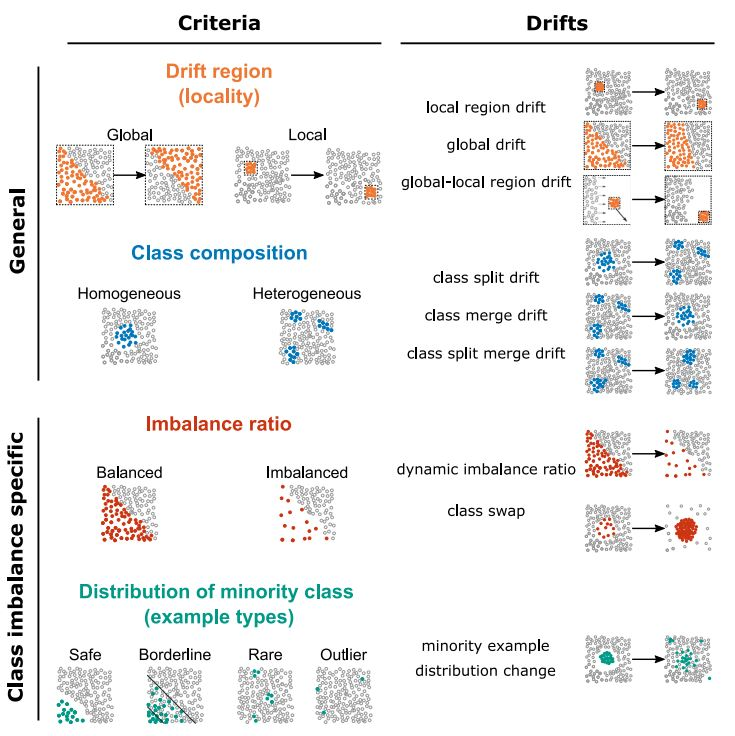
\includegraphics[width=15cm]{figures/drift_criteria.JPG}
    \caption{Rodzaje typów zmian obsługiwanych przez generator strumieni danych \cite{Article:TypyPrzykladow}}\label{Figure:DriftCriteria}
\end{figure}

\noindent Na rysunku \ref{Figure:DriftCriteria} przedstawiono problem klasyfikacji binarnej. Klasa mniejszościowa na przedstawionych ilustracjach została oznaczona odpowiednio kolorami: pomarańczowym, niebieskim, czerwonym oraz zielonym. Klasa większościowa na każdej z ilustracji została oznaczona kolorem szarym. Na podstawie rysunku można zobaczyć jak wyglądają operacje: podziału grupy klasy mniejszościowej na kilka mniejszych skupisk (\textit{class split drift}), połączenia grup klasy mniejszościowej w jedno większe skupisko (\textit{class merge drift}), zmiany liczności przykładów w danych klasach (\textit{dynamic imbalance ratio, class swap}), zmiany rozkładu danych poprzez napływ przykładów danego typu (\textit{minority example distribution change}) oraz przemieszania się skupisk w przestrzeni atrybutów (\textit{region drift}). 

\section{Proces generowania danych}

\noindent Wiedząc w jaki sposób osiągnąć określony typ zmian w strumieniu danych, kolejnym krokiem był proces wygenerowania wszystkich potrzebnych strumieni danych do nauki algorytmów. W tym celu zdecydowano się wygenerować wiele różnych przypadków zawierających różne typy zmian, które zostały opisane we wcześniejszej sekcji. Szczegółową konfigurację parametrów można przeanalizować z rysunku \ref{Figure:DriftParameters}.

\begin{figure}[h] 
    \centering
    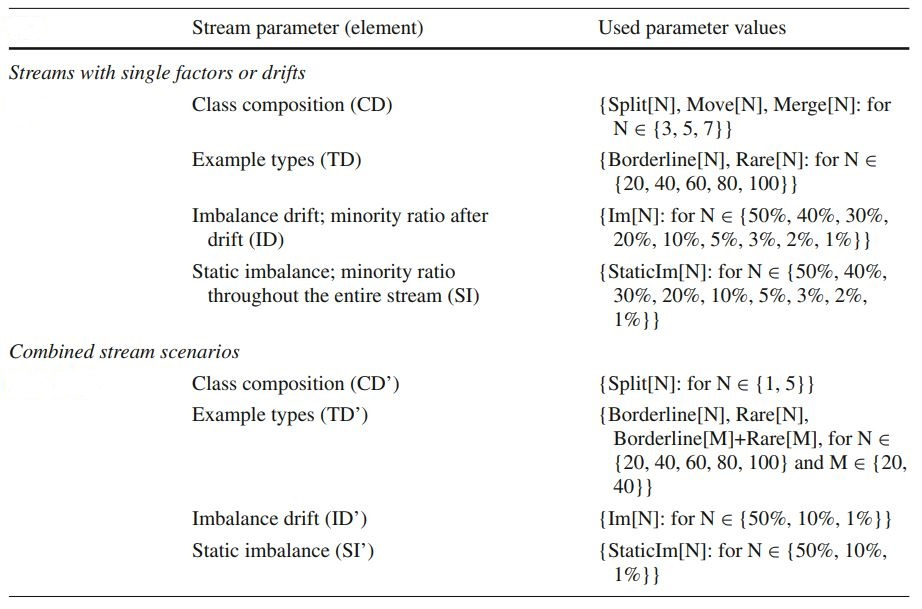
\includegraphics[width=15cm]{figures/drift_parameters.JPG}
    \caption{Wartości parametrów wykorzystanych do generacji strumieni danych \cite{Article:TypyPrzykladow}}\label{Figure:DriftParameters}
\end{figure}

\begin{figure}[h] 
    \centering
    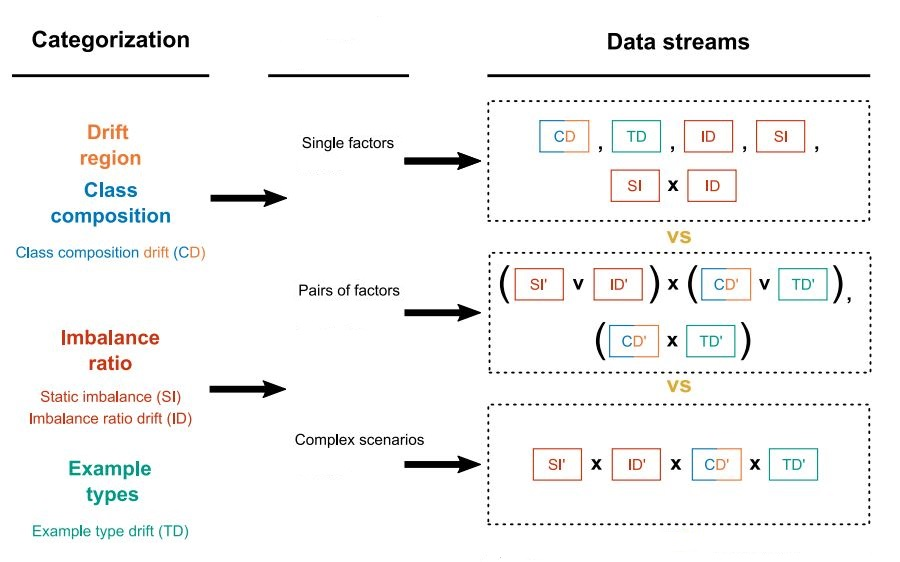
\includegraphics[width=13cm]{figures/drift_categorization.JPG}
    \caption{Wartości parametrów wykorzystanych do generacji strumieni danych \cite{Article:TypyPrzykladow}}\label{Figure:DriftCategorization}
\end{figure}

\noindent Jak można zauważyć z rysunku \ref{Figure:DriftCategorization}, w niniejszej analizie sprawdzone zostaną przypadki strumieni danych, które zawierają: jeden czynnik trudności (\english{single factors}), pary czynników trudności (\english{pairs of factors}) oraz złożone scenariusze zawierające wiele czynników trudności (\english{complex scenarios}). Taka analiza ma za zadanie wskazać, wśród określonych eksperymentów, typy zmian, z którymi algorytmy radzą sobie najgorzej, poprzez naukę na strumieniach z jednym aspektem trudności. Poza tym kolejnym celem jest przetestowanie, jak algorytmy radzą sobie ze strumieniami danych zawierającymi wiele aspektów trudności. Wygenerowane w ten sposób strumienie danych są dobrym odwzorowaniem rzeczywistych danych, które w rzeczywistości zawierają wiele czynników trudności, nieraz trudnych do zdefiniowania. W ten sposób będzie wiadomo, które algorytmy mogłyby sobie poradzić z analizą rzeczywistych danych i znalazłyby zastosowanie w dzisiejszym świecie.

\section{Przykładowe instancje wygenerowanych strumieni danych}

\noindent W ramach niniejszej sekcji przedstawione zostaną przykładowe instancje wygenerowanych strumieni danych wraz z wytłumaczeniem konwencji nazewnictwa, która jest wykorzystywana w dalszej części pracy. W ramach procesu generacji udało się stworzyć 381 różnych instancji strumieni danych biorąc pod uwagę różnego rodzaje typy zmian, które mogą zajść w strumieniu oraz możliwość zaistnienia kilku typów zmian jednocześnie. Warto też zwrócić uwagę na fakt, że każdy z stworzonych strumieni danych zawiera dokładnie 200 000 przykładów, gdzie każdy przykład opisany jest przez 5 atrybutów numerycznych oraz etykietę binarną. Jeżeli w strumieniu występuje dryf pojęć to jest to dryf stopniowy (\textit{incremental}), który ma miejsce od momentu przetwarzania przykładu numer 70 000 do momentu przetworzenia przykładu numer 100 000. Dodatkowo każda z klas, przed możliwym wystąpieniem dryfu, jest równoliczna (jeśli nie skorzystano z opcji \textit{StaticIm}) oraz wszystkie przykłady z klasy mniejszościowej oraz większościowej oznaczone są oznaczone jako typ \textit{Safe}. Jeden z przykładów z pracy \cite{Article:TypyPrzykladow} obrazujący podstawowe miary badanych strumieni można przeanalizować na rysunku \ref{Figure:DriftExample}.

\begin{figure}[h]
    \centering
    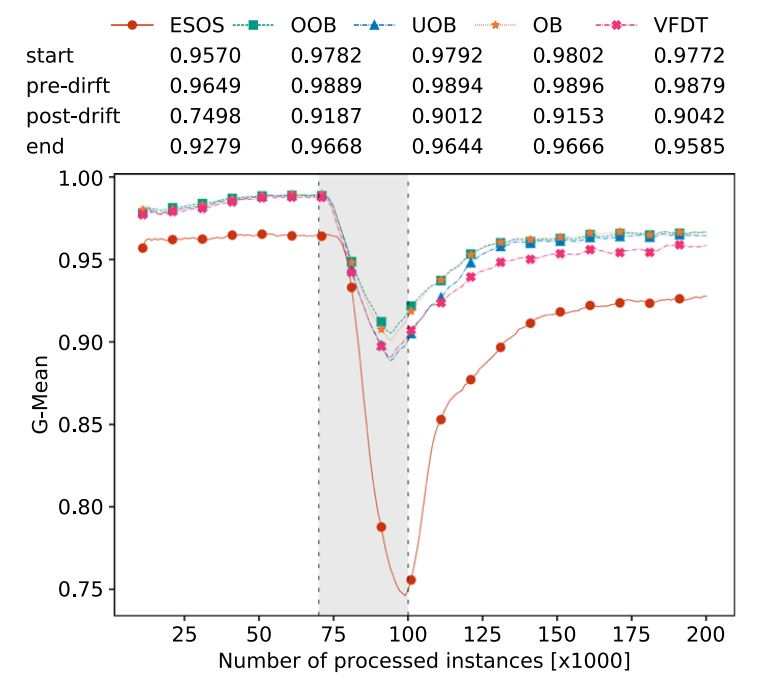
\includegraphics[width=13cm]{figures/drift_example.JPG}
    \caption{Ocena jednego z przykładowych strumieni danych zaprezentowanego w pracy \cite{Article:TypyPrzykladow}}\label{Figure:DriftExample}
\end{figure}

W dalszej części pracy będzie wykorzystywana określona konwencja nazewnictwa wygenerowanych strumieni danych. Wykorzystana konwencja została wytłumaczona poniżej na kilku przykładach wygenerowanych nazw:

\begin{itemize}
    \item \textit{Borderline20+Rare20} - oznacza napływ 20\% przykładów typu \textit{Borderline} i \textit{Rare} podczas zaobserwowanego dryfu
    \item \textit{Im1+Rare60} - oznacza napływ 60\% przykładów typu \textit{Rare} oraz zmianę liczności przykładów z klasy mniejszościowej na 1\% podczas zaobserwowanego dryfu
    \item \textit{Split5+Borderline40} - oznacza napływ 40\% przykładów typu \textit{Borderline} oraz podział skupiska przykładów klasy mniejszościowej na 5 mniejszych skupisk podczas zaobserwowanego dryfu
    \item \textit{StaticIm40+Im90} - oznacza, że na samym początku w strumieniu było 40\% przykładów z klasy mniejszościowej, gdzie po zaobserwowaniu dryfu wartość ta zmieniła się do 90\%
    \item \textit{Im10+Borderline40+Rare40} - oznacza napływ 40\% przykładów typu \textit{Borderline} i \textit{Rare} oraz zmianę liczności przykładów z klasy mniejszościowej na 10\% po zaobserwowaniu dryfu
    \item \textit{StaticIm10+Split5+Im1+Borderline40+Rare40} - oznacza napływ 40\% przykładów typu \textit{Borderline} i \textit{Rare}, zmianę liczności przykładów z klasy mniejszościowej z 10\% na 1\% oraz podział skupiska przykładów klasy mniejszościowej na 5 mniejszych skupisk
\end{itemize}